\chapter{Problem description }

The main objective was the assessment and improvement of some routines
used in the free energy package Transformato. A further goal was to
minimize the necessity of additional adjustments by the user, i.e.
reasonable mutation routes have to be generated automatically. The
proposed route should be directly usable for the further Transformato
workflow.

In a first step, the reliability of the current Transformato workflow
had to be assessed, for instance the quality of the proposed common
cores. Different settings for the construction of the maximum common
substructure have been compared. 

The order of the transformation steps has been optimized, especially
for the case of more complex mutation routes which occur for connected
dummy regions involving ring structures, multiple chains or various
atom types. 

Particularly intricate problems occur for ring structures. There are
some especially sensitive cases, e.g. ring breakage poses especially
difficult problems because it can lead to fast changes in free energy
and cause significant estimation error \cite{Liu.2015}. Neither should
the mutation of atoms generate vacancies in the inner part of the
molecule nor should opened rings remain longer than necessary and
a sufficiently systematic and - especially concerning rings - symmetric
processing of the nodes has to be performed. These rules have to be
implemented by maintaining the crucial constraint that no atoms are
detached from the main part encompassing the common core, i.e. no
disconnected components emerge under any circumstances.

Using a graph representation of the involved molecules, the construction
of the intermediates between the final states has been optimized.
New algorithms have been written in Python and subsequently integrated
into the existing Transformato package. Finally, the effect of different
algorithms on the efficiency of the free energy calculations had to
be validated by means of molecular dynamics simulations. 

To obtain a reliable test set of molecules, sdf-files of ligands have
been downloaded from PDB-BIND. These test molecules should cover a
broad range in size, complexity and potentially intricate compounds,
like polycyclic structures and highly branched chains.

\subsection{Used algorithms and software packages}

The Transformato package is written in Python. Therefore, Python packages
have also been used for molecule processing and graph representations.
The creation of molecule objects and the determination of the maximum
common substructure is done via rdkit\cite{key-3}. NetworkX\cite{AricA.Hagberg.2008}
provides functions for graph visualization and analysis. It is easily
possible to convert molecules created using rdkit into networkx graph-objects
and hence utilize the functions of networkx for the molecules and
common cores constructed. Particularly, graph traversal algorithms
like breadth-first and depth-first search can be easily implemented
(see below).

\section{Assessment of common core settings}

Rdkit allows the search of a maximal common substructure (which can
serve as common core for Transformato) via the \texttt{rdFMCS.FindMCS}-function.
Per default, the objective is to maximize the number of atoms, albeit
different settings, like maximize the number of bonds or ignoring
or equalizing specific atom types are available. At the moment, for
Transformato maximization of atoms and atom identity is used. If the
data comprises hydrogens, these are excluded before the common core
is calculated. As stated above, the presence of hydrogens can influence
the maximum common substructure heavily (fig. 4.1).

\begin{figure}

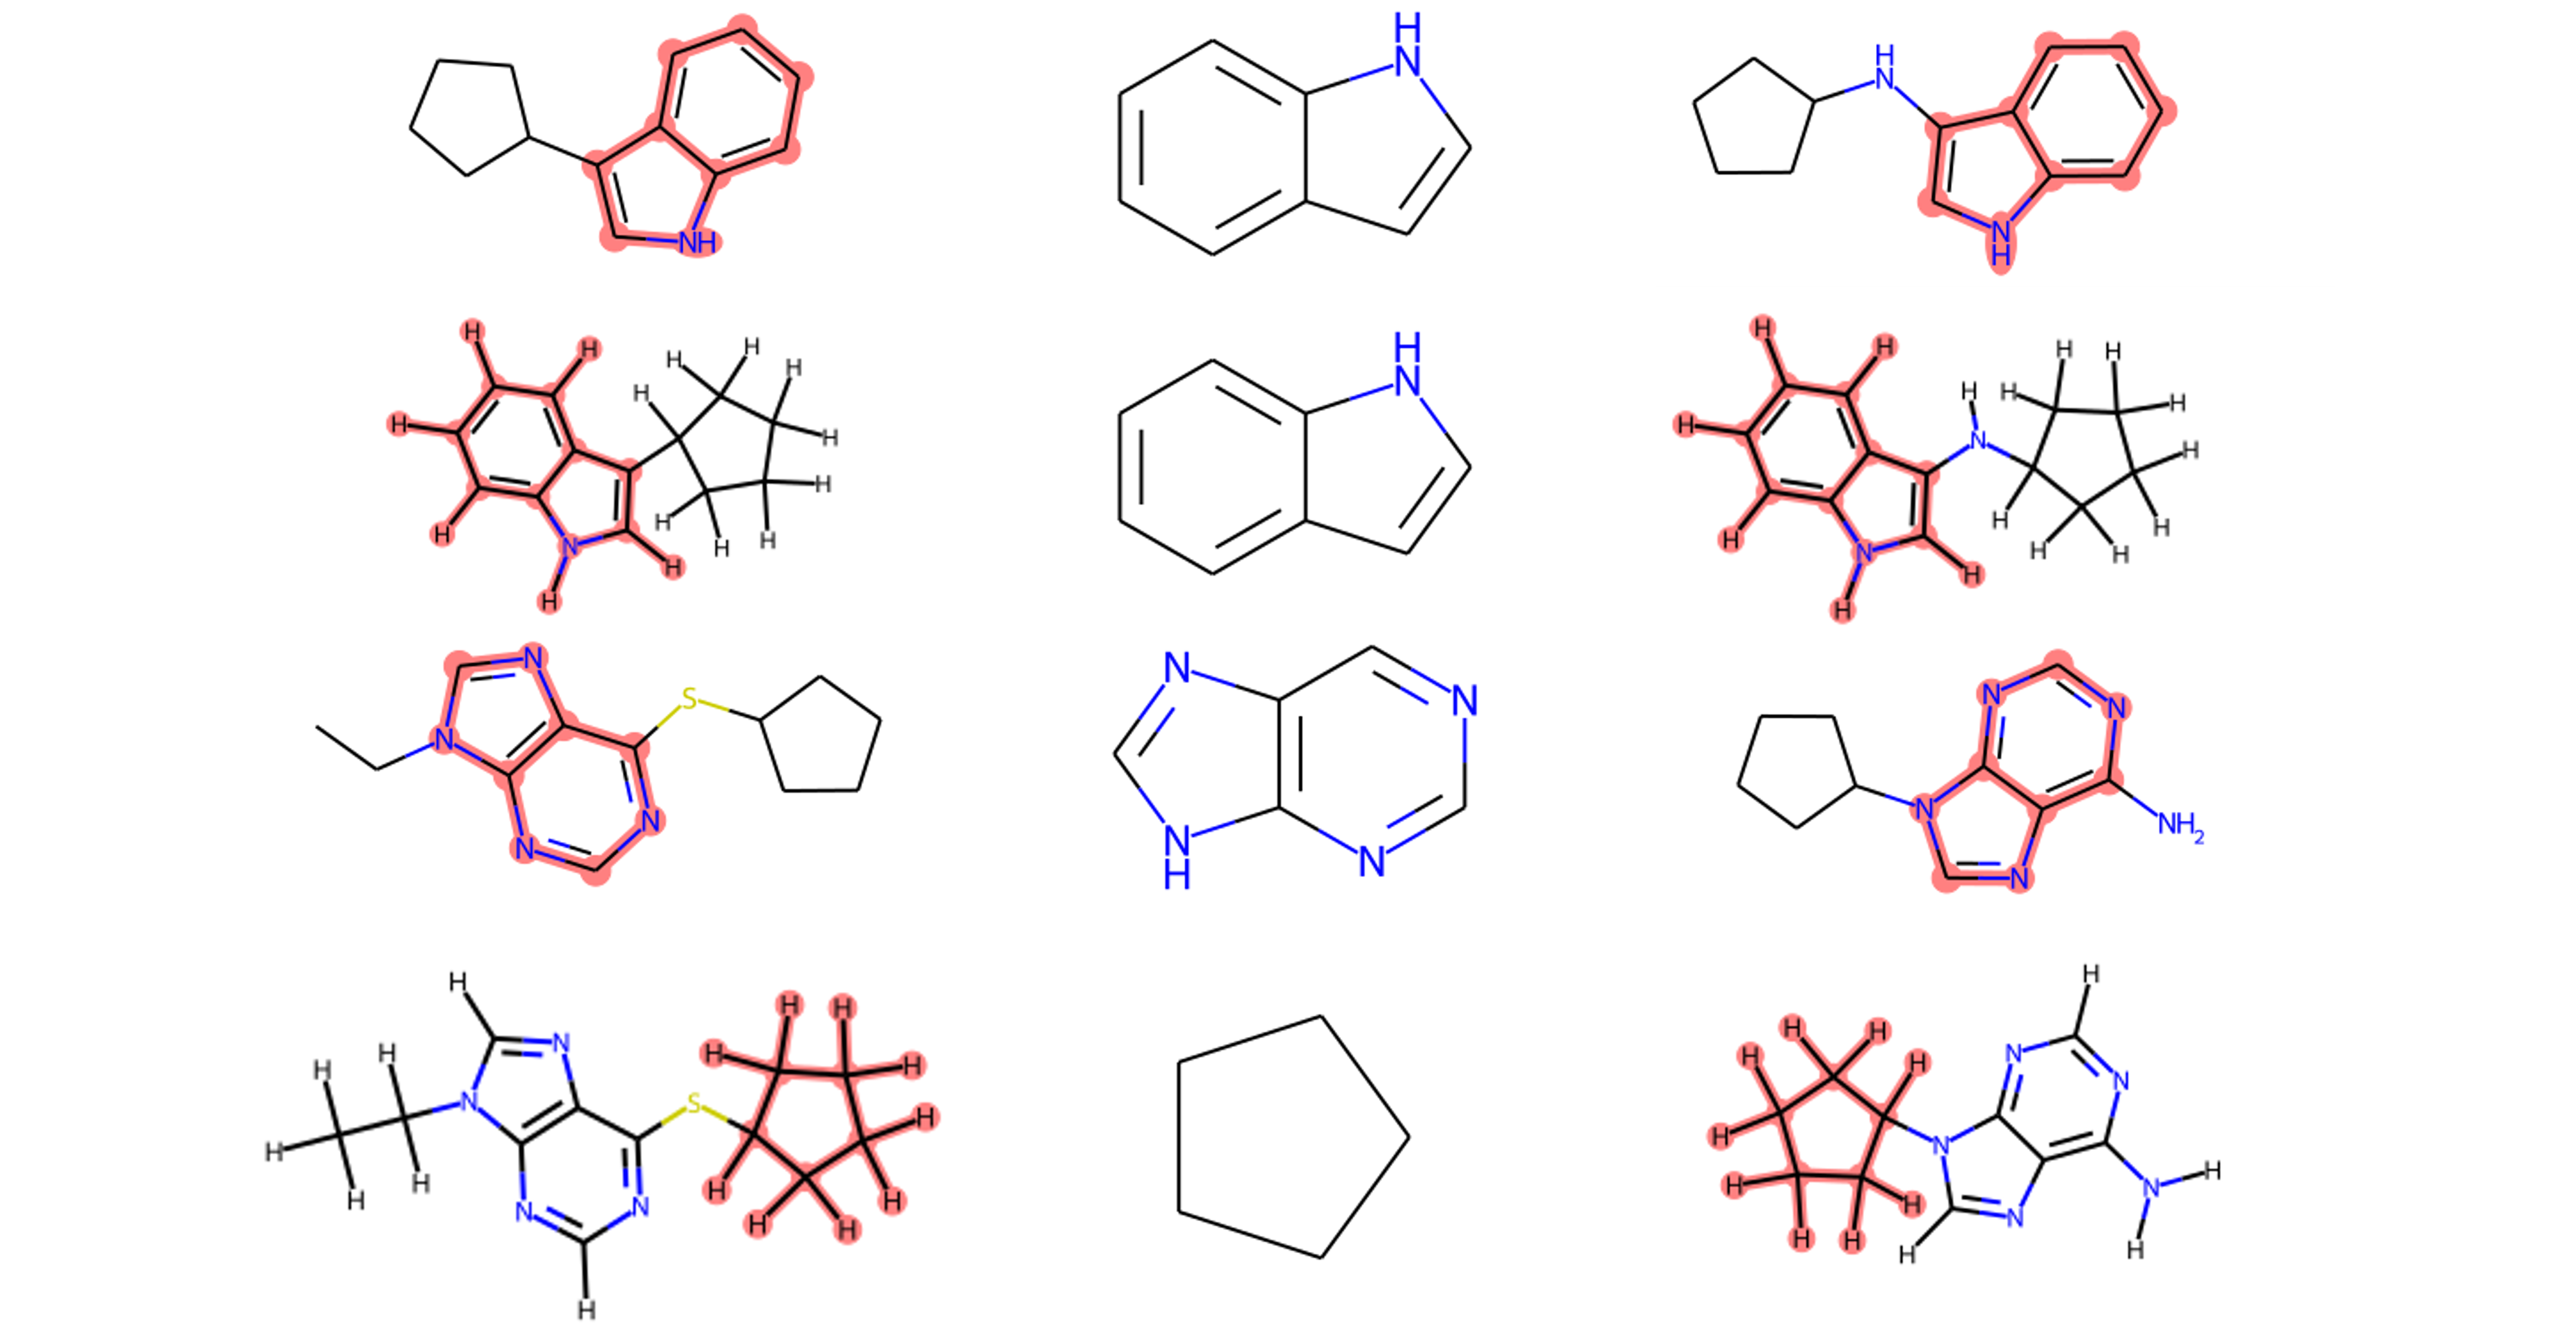
\includegraphics[scale=0.3]{hydrogens_plus_minus}\caption{left: molecule 1; middle: common core; right: molecule 2; the first
and the last two rows show the same molecules, in the upper row without,
in the lower with hydrogens, in case of the lower molecule combination
the common core changes when hydrogens are added to the Rdkit-molecule
representation }

\end{figure}

Settings concerning the allowed involvement of ring structures in
the common core are of crucial importance. Firstly, these parameters
can influence the common core construction drastically and, secondly,
can even be decisive if the generated common core is valid for the
Transformato workflow.

Important ring-related settings are ringMatchesRingOnly, completeRingsOnly
and the ringCompare-parameter. 

To obtain valid common cores for the processing of Transformato, ringMatchesRingOnly
and completeRingsOnly must be set to True: The former argument indicates
that ring atoms of one molecule are only matched against ring atoms
of the other molecule, the latter ensures that no partial rings are
involved in the common core. Especially the latter constraint is a
necessary condition for a valid common core. (Otherwise, if partial
rings take part of the common core, dummy regions will be inevitably
connected to the common core via multiple bonds.)

The ringCompare-parameter parameter accepts the StrictRingFusion-argument.
It imposes that in case of multiple rings aromaticity is properly
taken into account. Fig. 4.2 illustrates the effect of the parameters
on the common core of two cyclic example molecules. However, enforcing
of StrictRingFusion can still lead to maximum common substructures
which are not valid Transformato common cores because a dummy region
is connected via multiple ring atoms of the same ring with the common
core.

(It seems to be advisable to warn the user in this case that the common
core does not fit the expectations of the Transformato workflow. Alternatively,
one could check after the creation if the common core is valid. If
it is not, one could for instance search for a new common core encompassing fewer
atoms until a valid common core is found. 
Alternatively, one could prohibit the involvement of ring atoms for this particular
molecule combination.
Probably the most efficient solution would be to remove the rings which contain atoms which participate in the partial ring causing the invalid common core from the representation used for creating the maximum common substructure and afterwards start a new search for a valid common core.
(Of course,
in the worst scenario, i.e. if both molecules only consist of ring-participating
atoms, no valid common core is conceivable.)
At the moment, the mutation algorithms presented below can deal with such invalid common cores. A helper function arbitrarily chooses one of the connections between common core and dummy region and the other ones are ignored for the mutation path.


\begin{figure}
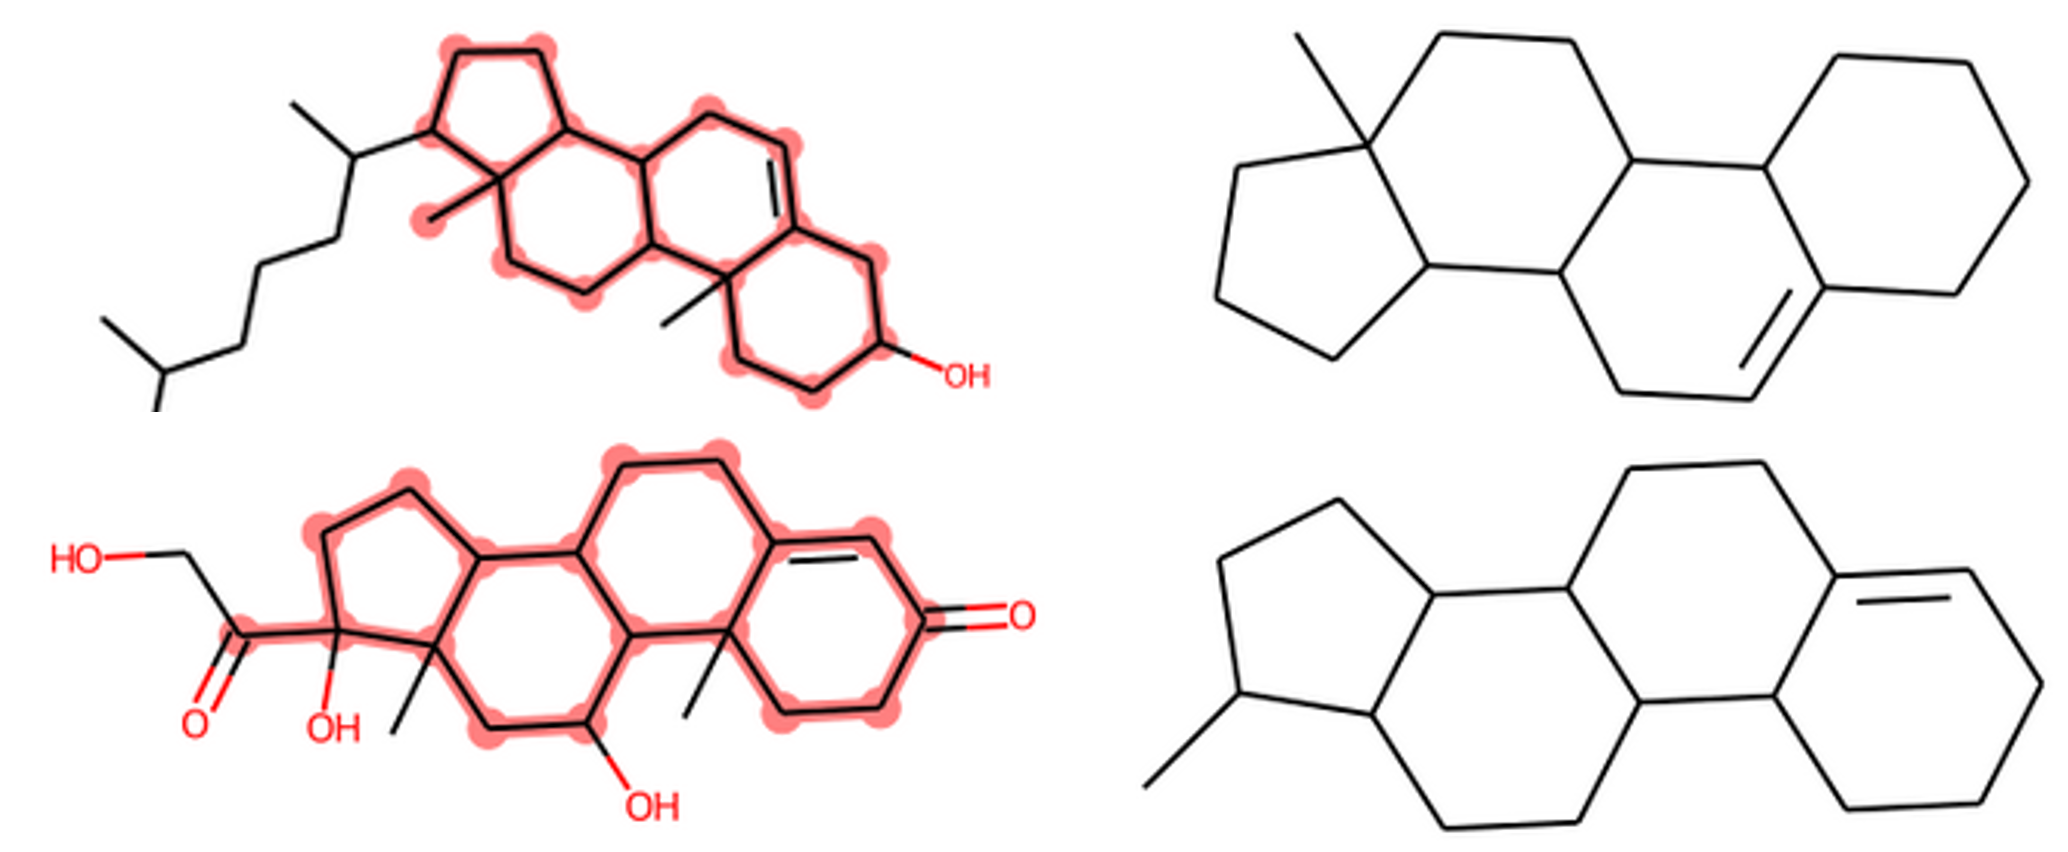
\includegraphics[scale=0.4]{sterols_wo_strictfusion}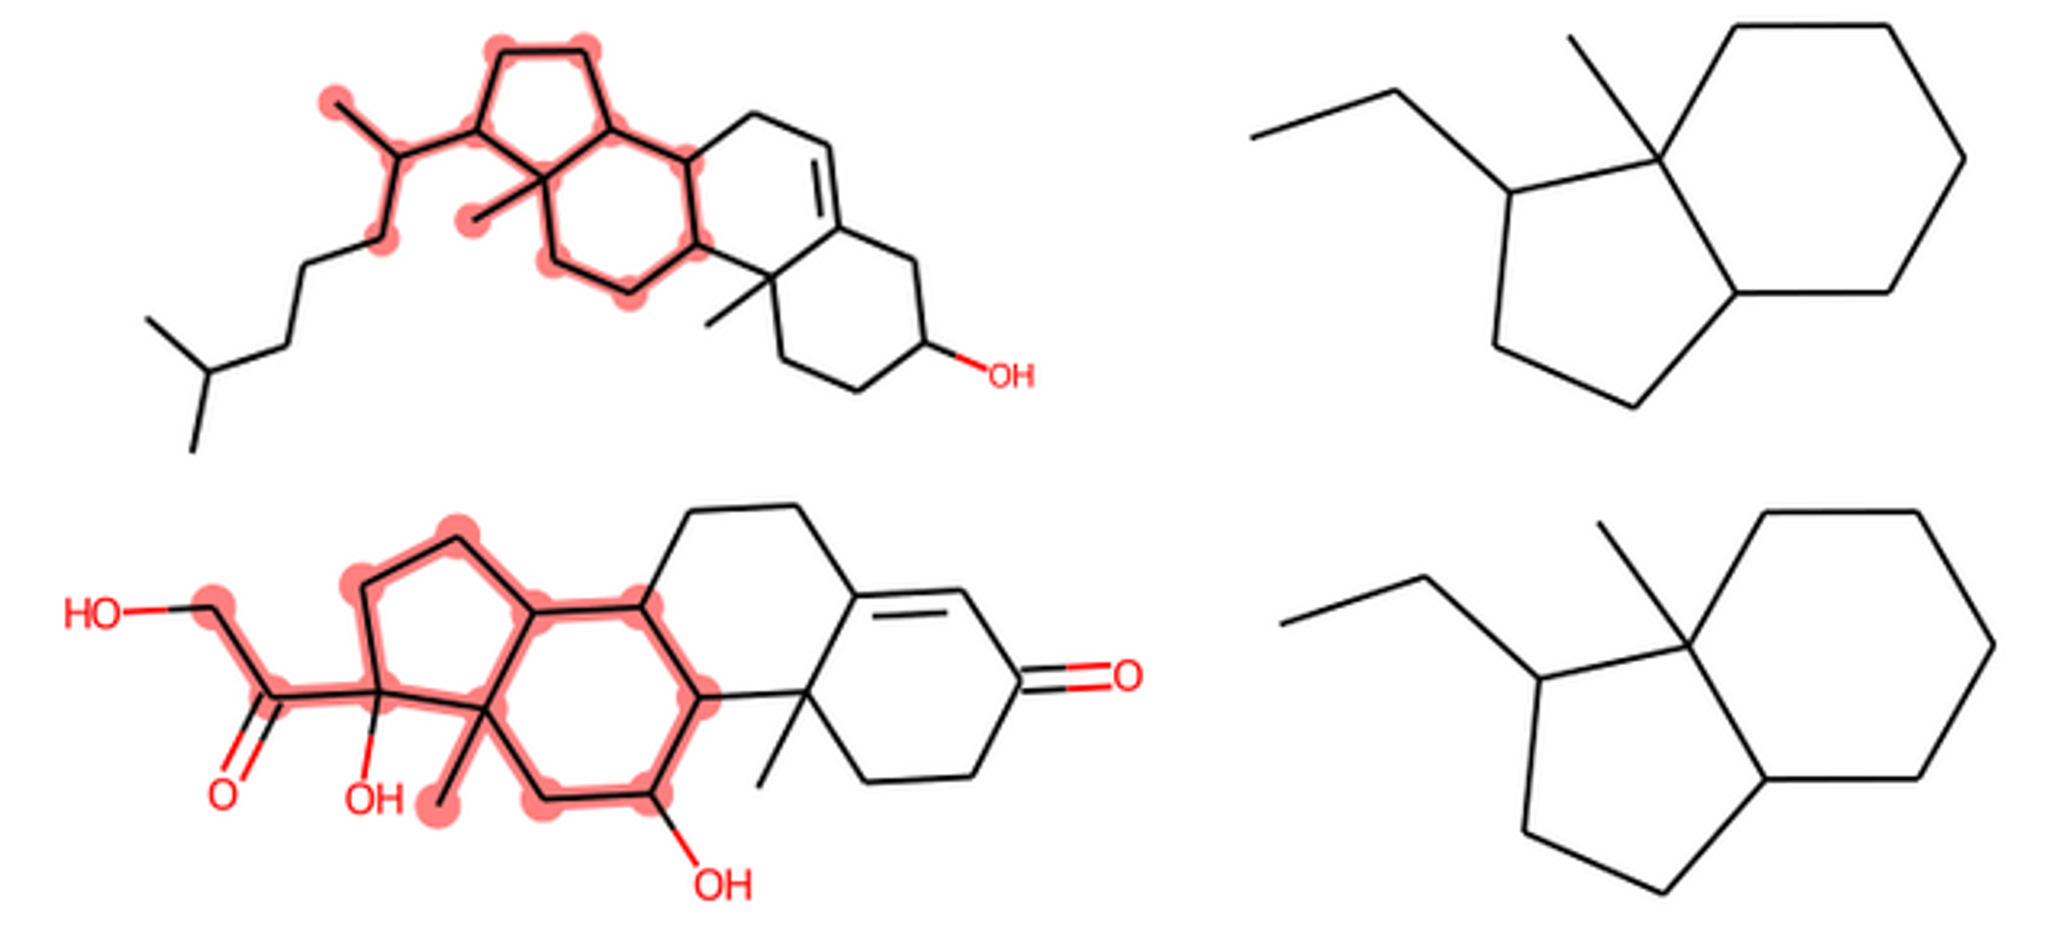
\includegraphics[scale=0.4]{sterols_w_strictfusion}

\caption{First and second column: Common core of two molecules (cholesterol
and cortisol) without strict fusion; third and fourth column: Common
core of two molecules with strict fusion }

\end{figure}


\section{Graph algorithms}

Using Networkx and Rdkit, the molecules and their common core are
represented as graphs (in which nodes indicate atoms and edges bonds
between them). The selection of the optimal mutation route can be
understood as a graph traversal problem in which the constraints mentioned
above are either implemented via the weights of the edges or sorting.
Hence the main task was to find suitable algorithms and graph initializations
to ensure an optimal processing of the mutation path.

Depth First Search (DFS) follows each chain of the graph as long as
possible, i.e. until a leaf node is reached. In contrast, Breadth
First Search (BFS) explores all chains simultaneously.\cite{Even.2012}
(Problems and differences of both algorithms are illustrated using
several examples below.)

In each of the algorithms implemented, the graph traversal starts
with the node which connects dummy region and common core as the root.
Shortest paths to all nodes of the dummy region are determined.

\begin{figure}

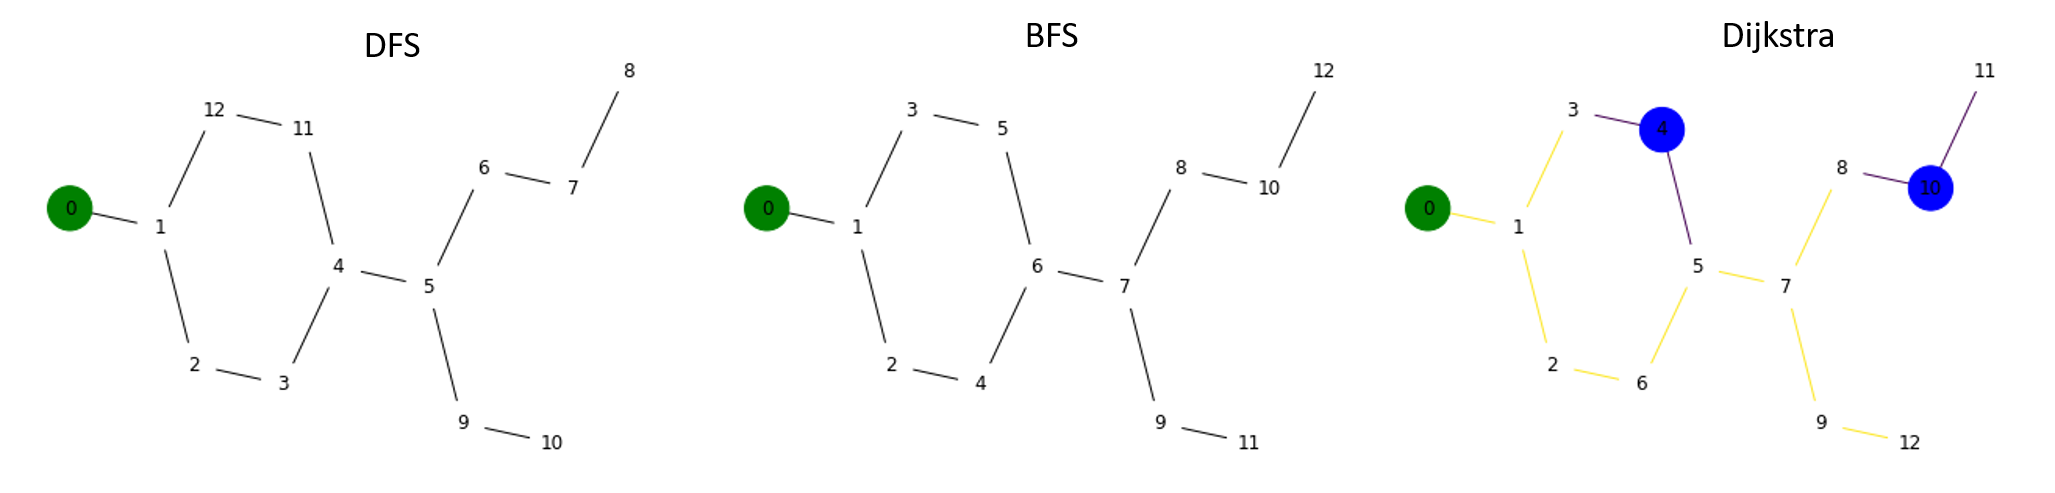
\includegraphics[scale=0.45]{dfs_bfs_dijkstra_comp1}\caption{Comparison of different graph traversal algorithms; left: depth first
search; middle: breadth first search; right: Dijkstra algorithm, the
edges connecting blue colored nodes have increased weights leading
to a mutation route differing from BFS; the final processing of the
nodes happens in reversed order}

\end{figure}

As the longest shortest path pertains to the node which has the greatest
distance from the root (i.e. the atom with greatest distance from
the common core), the list of mutations orders has to be reversed.

If weighted graphs are used, the Dijkstra algorithm can be applied.
It finds the shortest path between two nodes or between a root node
and all other nodes of the weighted graph (the weights indicate the
edge length from one node to the other one) . For unweighted graphs
(or, equivalently, graphs with uniform weights), the Dijkstra algorithm
reduces to BFS. Fig. 4.3 shows the different routes for modified weights.
(In the test cases presented below, graphs with uniformly weights
are initialized.)

\section{Added functionality}

\subsection{Functions}

To use the newly implemented mutation algorithms, initially the graph
is endowed with weights stored in a dictionary. The simulations shown
below use uniform weights, however it is possible to modify them to
enforce a certain mutation route (e.g. accelerating or postponing
the exclusion of specific heteroatoms). 

The Dijkstra algorithm is implemented via the \texttt{single\_source\_dijkstra}-function
of networkx.

The core functionality is given by the mutation processing functions.
At the moment, three such functions are implemented, additional to
the simple DFS-approach which leads to undesired outcomes. These functions
can be further modified by passing arguments which activate some helper
functions (see below).

The four main functions are: 

\texttt{\_calculate\_order\_of\_LJ\_mutations:} naive DFS 

\texttt{\_calculate\_order\_of\_LJ\_mutations\_new:} BFS/djikstra-algorithm
applied once for route

\texttt{\_calculate\_order\_of\_LJ\_mutations\_new\_iter:} BFS/djikstra-algorithm
applied iteratively, i.e. after each removal of an atom 

\texttt{\_calculate\_order\_of\_LJ\_mutations\_new\_iter\_change:}
works iteratively, i.e. after each removal of an atom, algorithm is
chosen depending on current state

\texttt{\_calculate\_order\_of\_LJ\_mutations }has already been implemented
in Transformato, but computes defective mutation routes and hence
should only be used for test purposes. The other three algorithms
are new and, in any case, resolve most of the problems of the earlier
algorithm (especially isolated removal of ring atoms).

Helper functions like cycle\_checks carry out tasks to ensure the
desired mutation route, e.g. count the number of cycles an atom participates
in. Further features of all algorithms are 'preferential removal',
i.e. if two atoms would have the same priority (given by the current
weight) for the next mutation step, the weight of the atom which is
next to an already removed atom is updated so that this atom is excluded
next.

\texttt{cycle\_checks(G)}: this function checks which atoms participate
in how many cycles/rings and returns a dictionary with the atoms as
key and the number of rings the atom is participating in as value
and a dictionary with the degree (i.e. number of edges) of each atom
node. It is currently used in \texttt{\_calculate\_order\_of\_LJ\_mutations\_new}
(via the \texttt{change\_route\_cycles}-function).

\texttt{change\_route\_cycles}(route, cycledict, degreedict, weightdict,
G): this function is used in \texttt{\_calculate\_order\_of\_LJ\_mutations\_new}
and sorts nodes according to degree, cycle participation and information
of nodes to be removed immediately before. The preliminary mutation
path is sorted using cycle and degree dictionary if nodes have same
weight (i.e. distance from root), the node participating in more cycles
is removed later if nodes have same weight (i.e. distance from root)
and same cycle participation number, the node which has more neighbours
already removed is removed earlier

\texttt{cycle\_checks\_nx}(G): This function modifies the weight of
the graph, nodes participating in many cycles get lower weight. It
is currently used in \texttt{\_calculate\_order\_of\_LJ\_mutations\_new\_iter}
and \texttt{...\_new\_iter\_change.} It returns a nx-graph-object
with updated weights (according to cycle participation of the atom).

\texttt{order\_checks\_nx}(G, removearray, G\_total): This function
performs the 'preferential removal', if a node is connected to the
node removed in the last step, its weight get a small increase so
that the removal of this node is prioritized. It is currently used
in\texttt{ \_calculate\_order\_of\_LJ\_mutations\_new\_iter} and returns
a nx-graph-object with updated weights.

If the cyclecheck-argument of the new mutation algorithms is True,
updates are updated according to cycle participation (as the systematic
processing of ring structures is one of the central goals, this argument
should always be set to True, except for comparison and test purposes).
If in the case of \texttt{\_calculate\_order\_of\_LJ\_mutations\_new
and \_calculate\_order\_of\_LJ\_mutations\_new\_iter} also ordercycles
or ordercheck, respectively, is set to True, weight updating according
to preferential removal decides that the node in which neighbourhood
nodes already have been turned off is removed next if there is no
possibility to decide between two nodes - i.e. the weight of both
would be exactly the same.

In each algorithm, all nodes of the graph (i.e. atoms) are usually
initialized with the same weight (e.g. 5). Alternatively, the user
could also pass a individual dictionary with different weights for
each atom type.

The BFS- / Dijkstra-algorithm starting from the node connecting common
core and dummy region is applied via the networkx-function \texttt{single\_source\_dijkstra}
which determines the path length of all dummy nodes to the root.

The main difference between these algorithms is that in \texttt{\_calculate\_order\_of\_LJ\_mutations\_new\_iter}
and \texttt{...\_iter\_change} the graph traversal part performed
using the Dijkstra algorithm is applied after each exclusion step
(i.e. $n!$ atoms are visited instead of $n$; even for large molecules
the additional computational cost is negligible, even in comparison
to the computational time the creation of the common core needs).
This has the advantage that after each mutation step weights can be
updated or even the search algorithm modified. 

The latter option allows for different mutation strategies depending
on the current state. This is demonstrated in \texttt{\_calculate\_order\_of\_LJ\_mutations\_new\_iter\_change}.
In contrast to the other algorithms, the algorithm processes information
if the last removed node was part of a chain or a cycle. Depending
on the state, the chain or cycle is processed fully before the algorithm
moves on to other parts of the molecule. Fig. 4.5 demonstrates the difference between both iter-algorithms.
Whereas in the non-iterated algorithm the found mutation route has to be reversed (since the atom node with the highest distance from the root is the first which has to be turned off), in the iterated versions at each iteration the node with the highest distance is added to an array which determines the final mutation route.

The computed mutation routes can be visualized directly via rdkit.
The route is represented by a colour gradient used for the atoms involved
in the mutation process (\texttt{\_show\_common\_core\_gradient}). 

Furthermore, an animated 3D-visualization of the mutation process
is implemented using py3Dmol (\texttt{animated\_visualization\_3d\_v2})\cite{key-4}. 

\begin{figure}
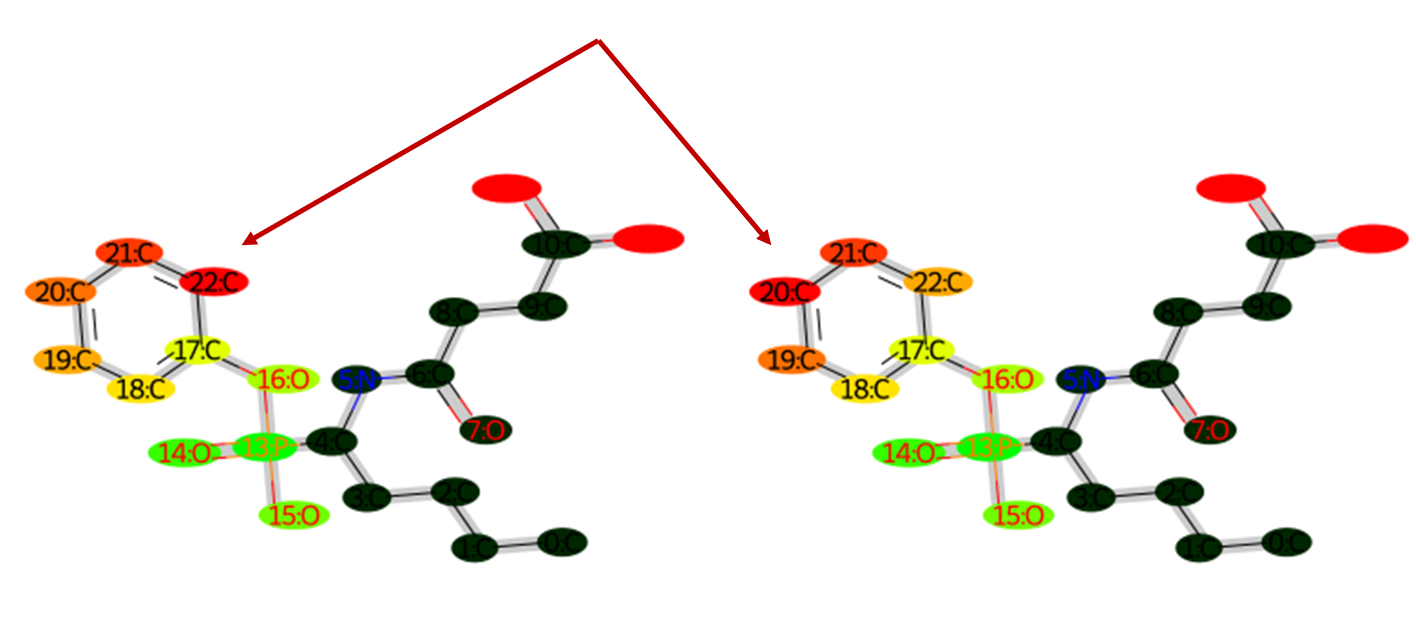
\includegraphics[scale=0.4]{simple_ring_exampledfs.png}

\caption{left: dfs-algorithm; right: bfs-algorithm; common core in dark; dfs
starts at carbon 22 and thus ring breakage gives rise to one long
chain which is processed subsequently, whereas bfs starts at carbon
22 and the two emerging chains are processed in a symmetric fashion
}

\end{figure}


\subsection{Examples for processing molecules}

\begin{figure}
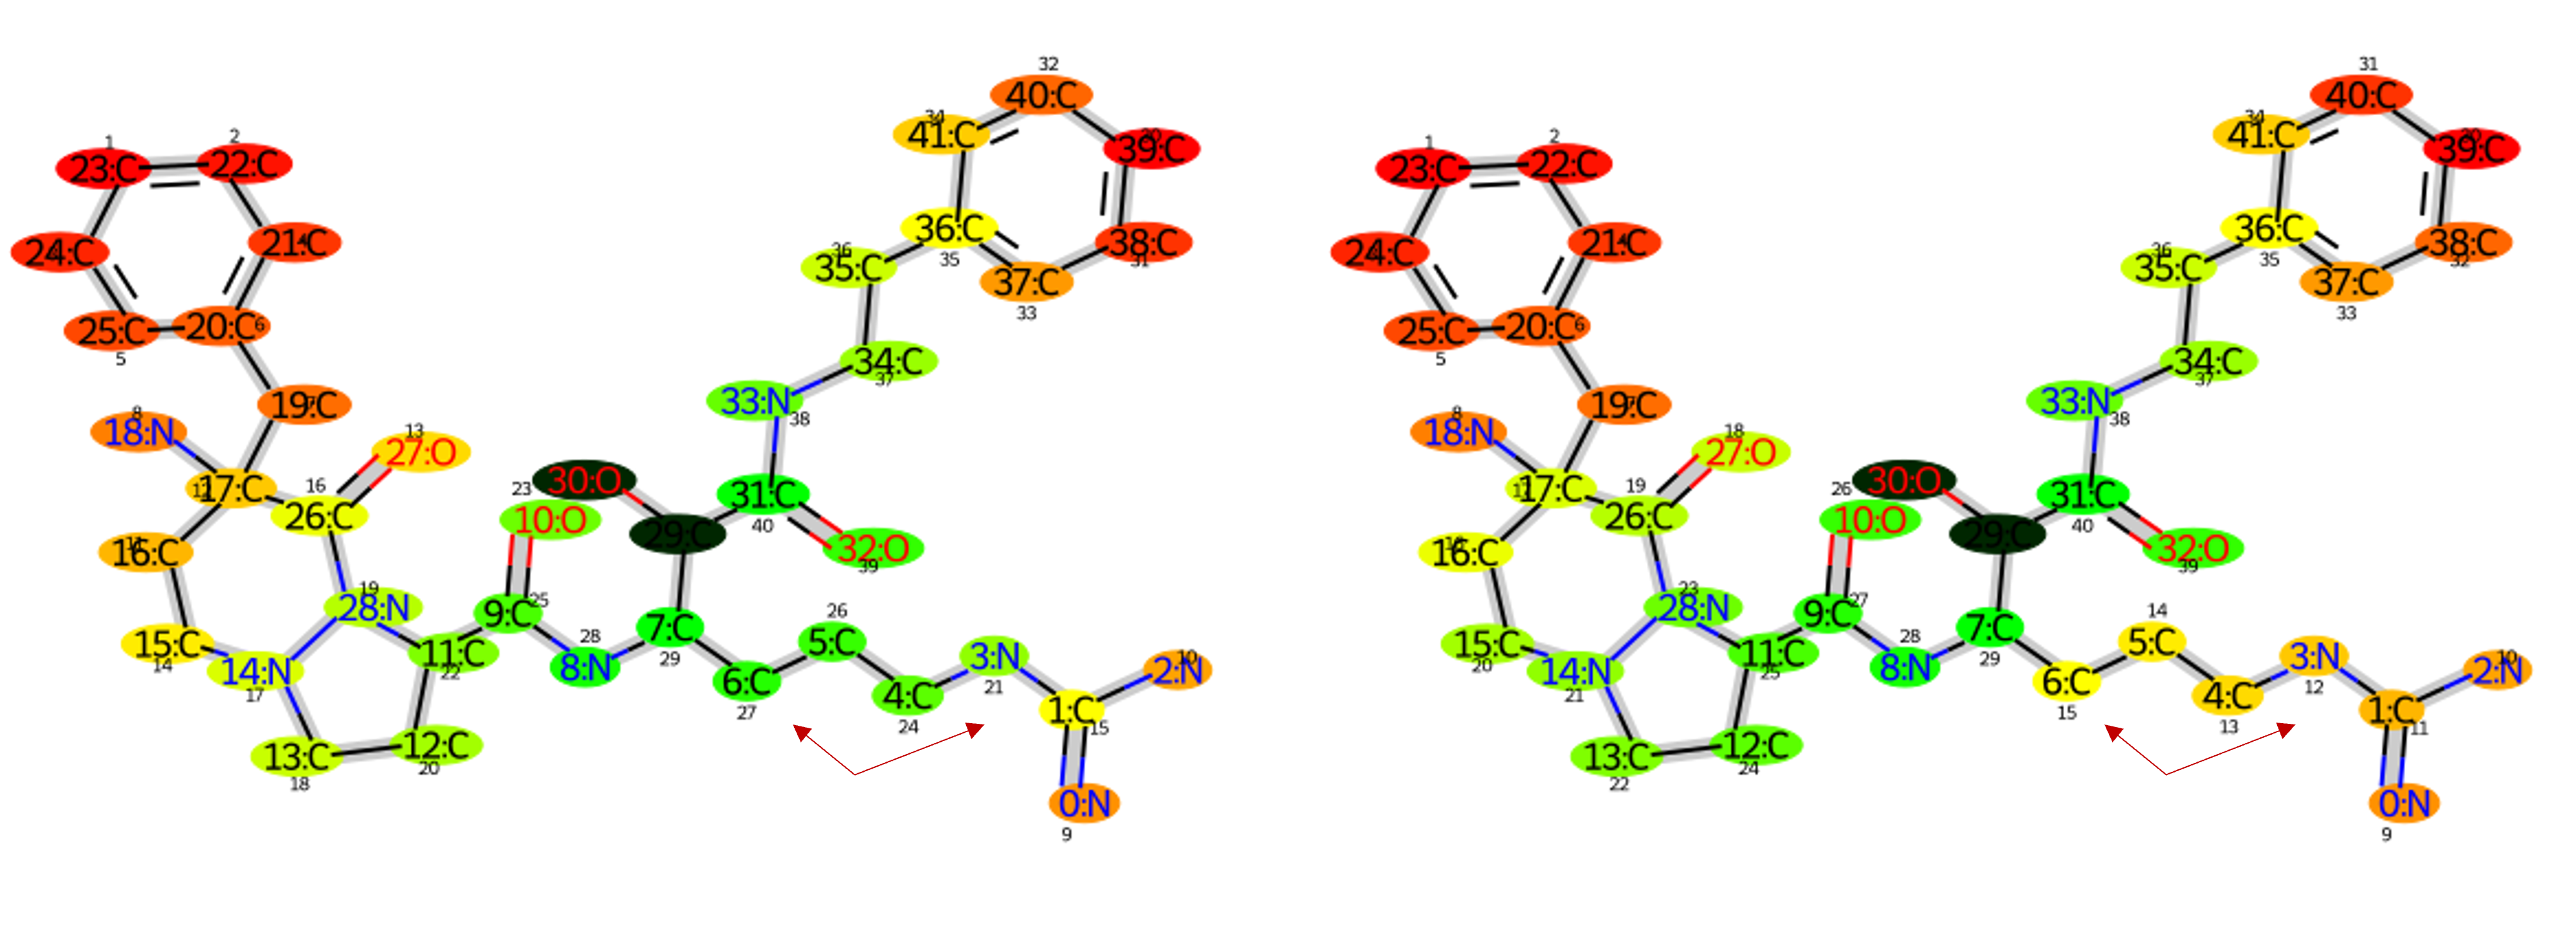
\includegraphics[scale=0.3]{iter_iter_change_1a5g_1}

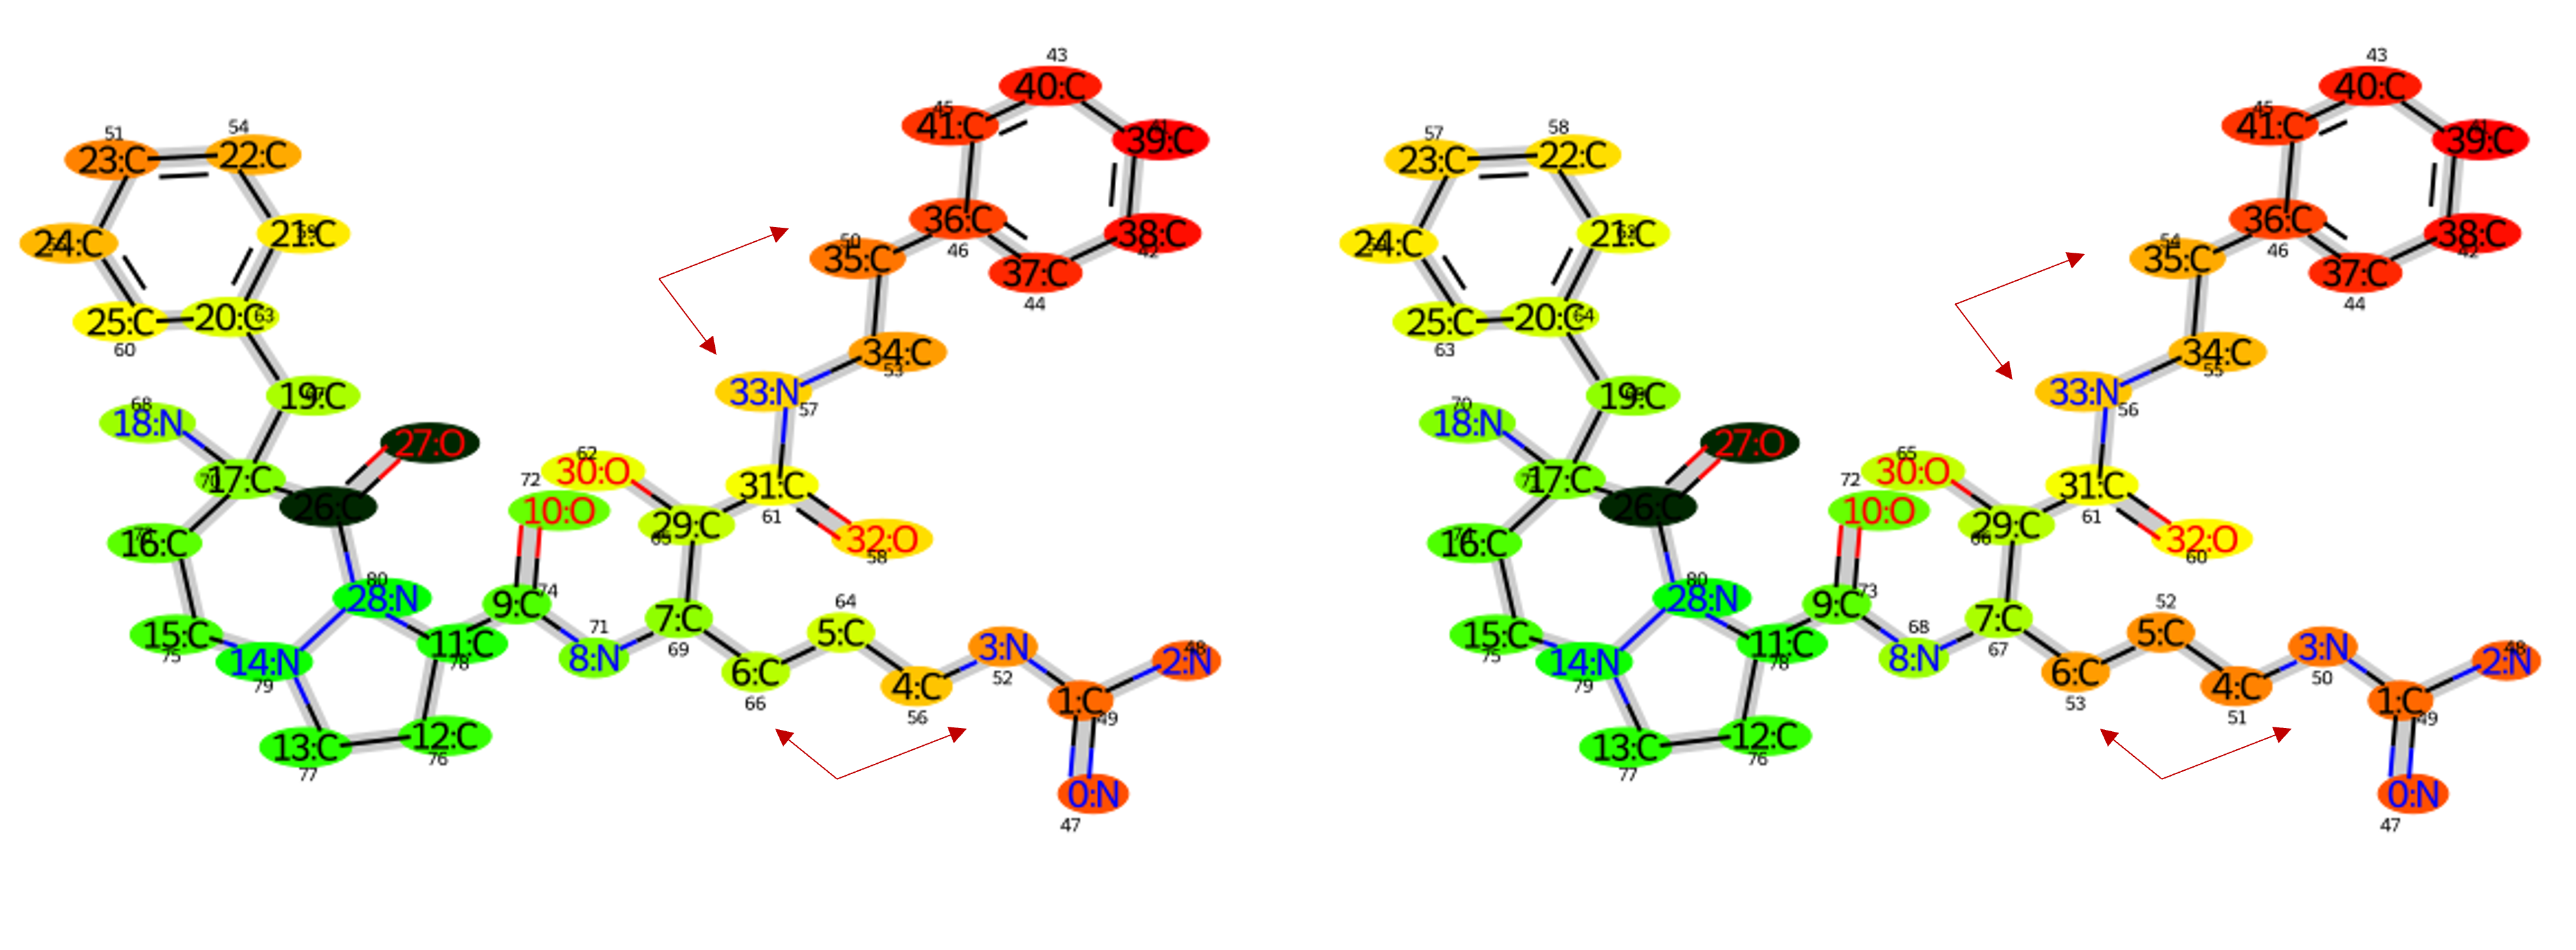
\includegraphics[scale=0.3]{iter_iter_change_1a5g_2}\caption{Example for the differences between iter- and iter\_change-algorithm;
left: iter; right: iter-change; iter-change processes all atoms within
a chain or a ring at once (if possible) before switching to other
parts of the molecule}
\end{figure}

For single rings, BFS (Dijkstra) automatically processes the atoms in the most symmetric way starting at the atom with the highest distance from the root (fig 4.4).
In more complex molecules, the systematic exploration of chains in
depth first search inevitably leads to big local gaps in processing
of the molecules. Fig. 4.6 shows this problem for a benzol ring which
is directly attached to the common core. As DFS goes along one path
until the end, i.e. a leaf node is reached, only four atoms of the
ring are visited at the beginning, whereas the remaining two are explored
last. Therefore, these two atoms are turned off first, but then the
algorithm continues at a wholly different location and the remaining
ring atoms persist in the system until the end of the mutation process.
In this case, BFS automatically produces the desired result. 

Similarly, in fig. 4.7 one atom of the ring (marked by the red circle)
is omitted in the first exploration using DFS.

As fig. 4.8 shows, also the processing of substituents is affected.

Multiple rings pose special problems for the mutation algorithms because
the processing of one of the rings can easily led to gaps in the adjacent
ones. Fig. 4.9 and 4.10 show that using DFS aggravated problems occur.
As in the case of one ring, the exploration route implies that one
of the rings is opened in a way that it gives rise to a lengthy chain.
However, it can even happen that the atom explored atom participates
even in two or multiple rings, so that both ring structures are opened
and teared apart (fig. 4.9). Alternatively, one half of each of the
rings is turned off first (fig. 4.10). 

\begin{figure}
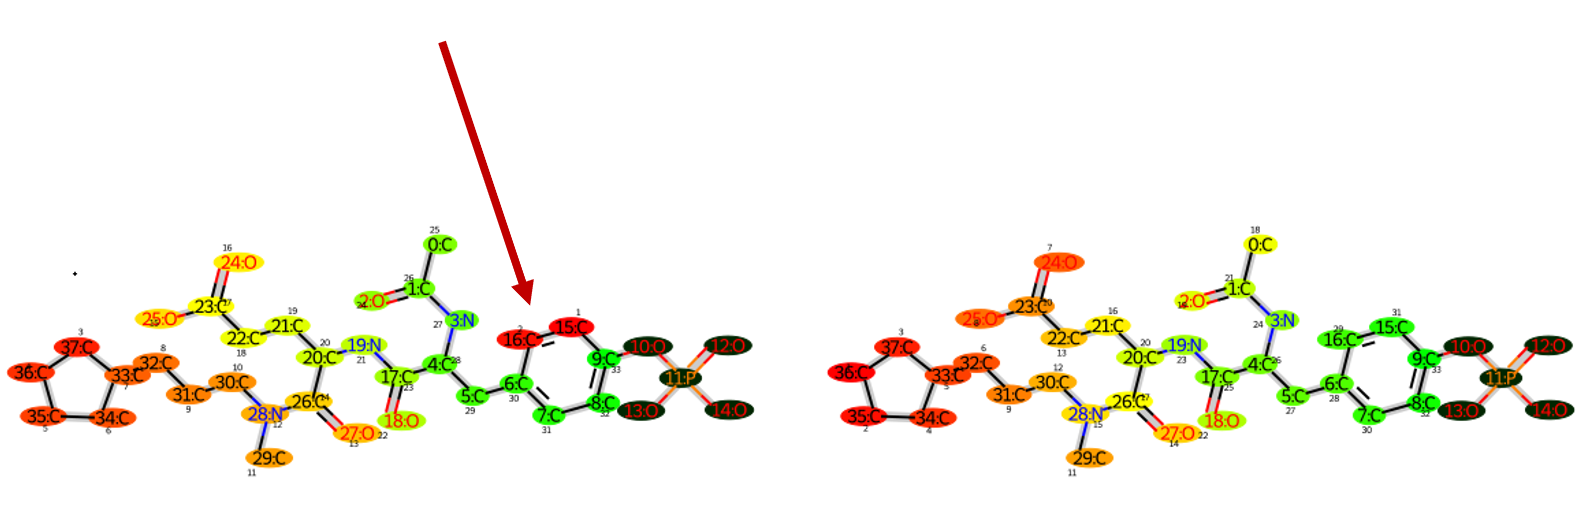
\includegraphics[scale=0.4]{simple_ring_exampledfs2}\caption{left: dfs-algorithm; right: bfs-algorithm; common core in dark; the
red arrow indicates the undesired processing of the ring atoms}

\end{figure}

\begin{figure}
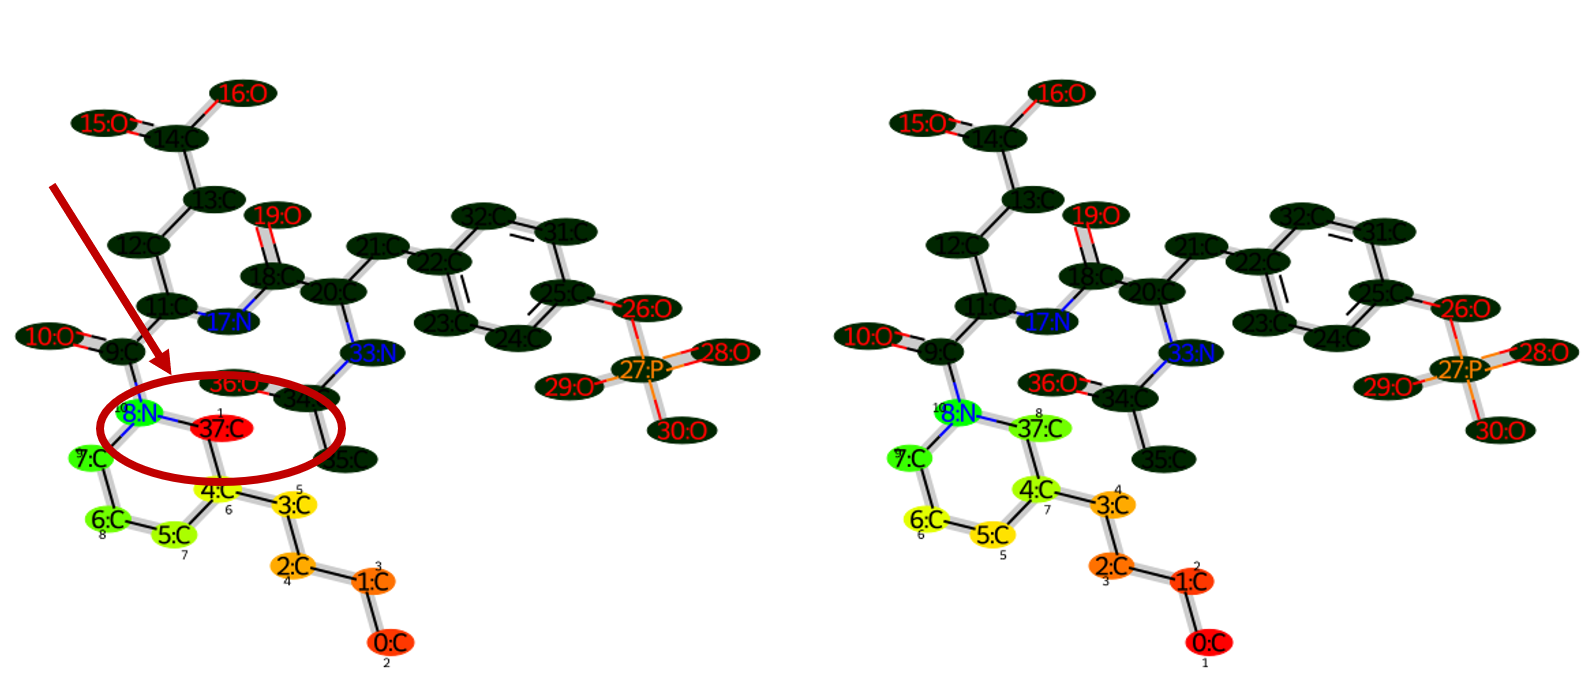
\includegraphics[scale=0.4]{simple_ring_exampledfs3}\caption{left: dfs-algorithm; right: bfs-algorithm; common core in dark; the
red arrow and circle indicates the undesired processing of the ring
atoms}

\end{figure}
\begin{figure}

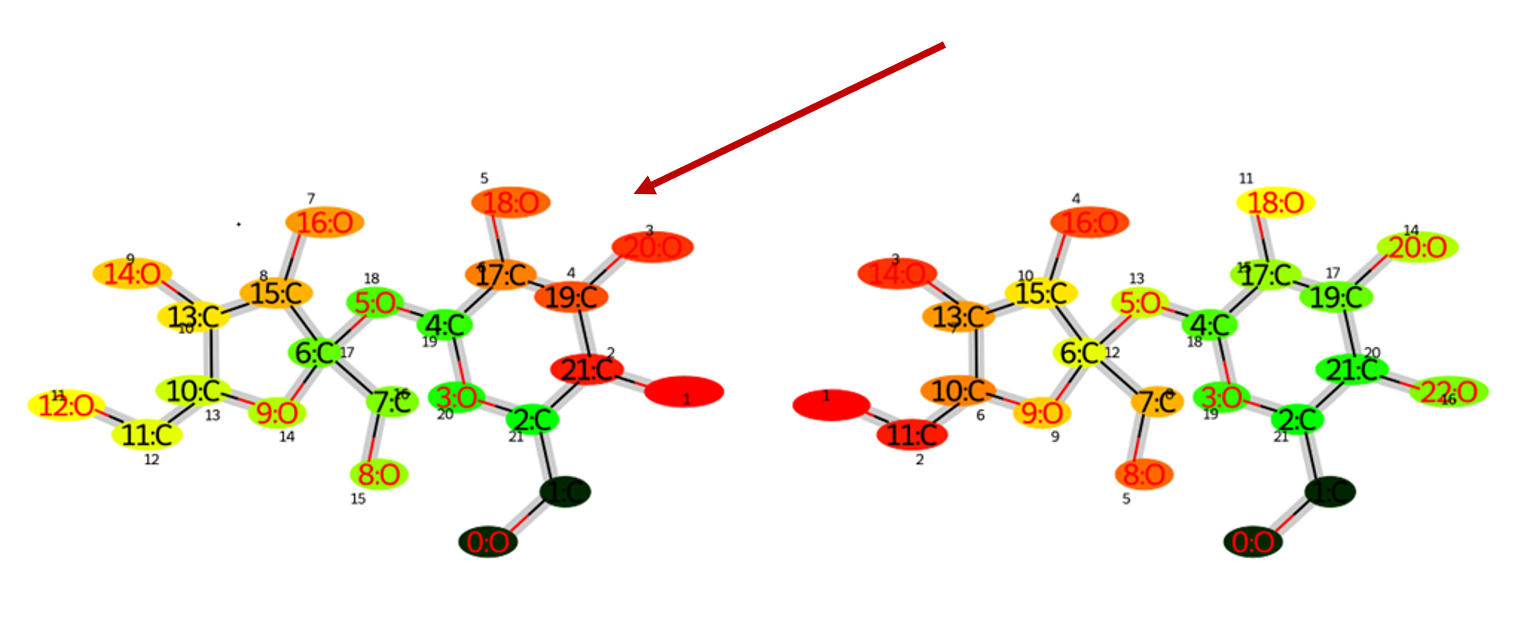
\includegraphics[scale=0.4]{simple_ring_exampledfs4}\caption{left: dfs-algorithm; right: bfs-algorithm; common core in dark; the
red arrow indicates the undesired processing of the ring atoms}

\end{figure}

\begin{figure}

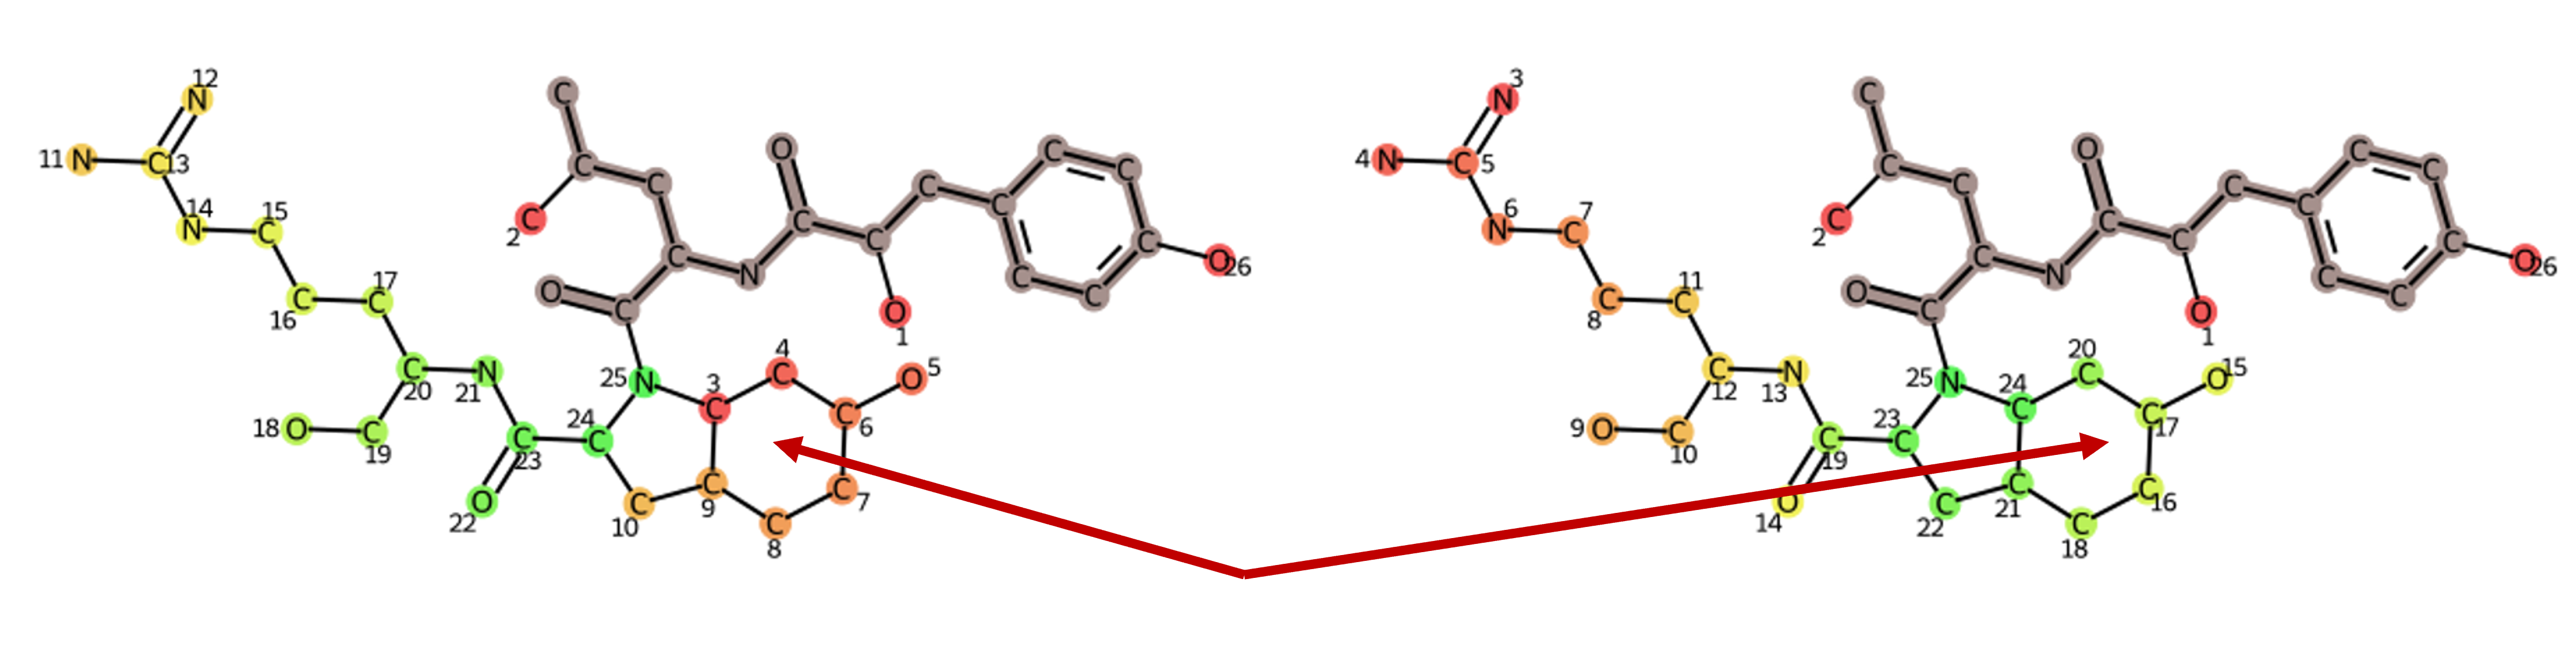
\includegraphics[scale=0.4]{2ring_example}\caption{left: dfs-algorithm; right: bfs-algorithm; common core in dark; the
red arrow indicates the undesired processing of the ring atoms}

\end{figure}

\begin{figure}

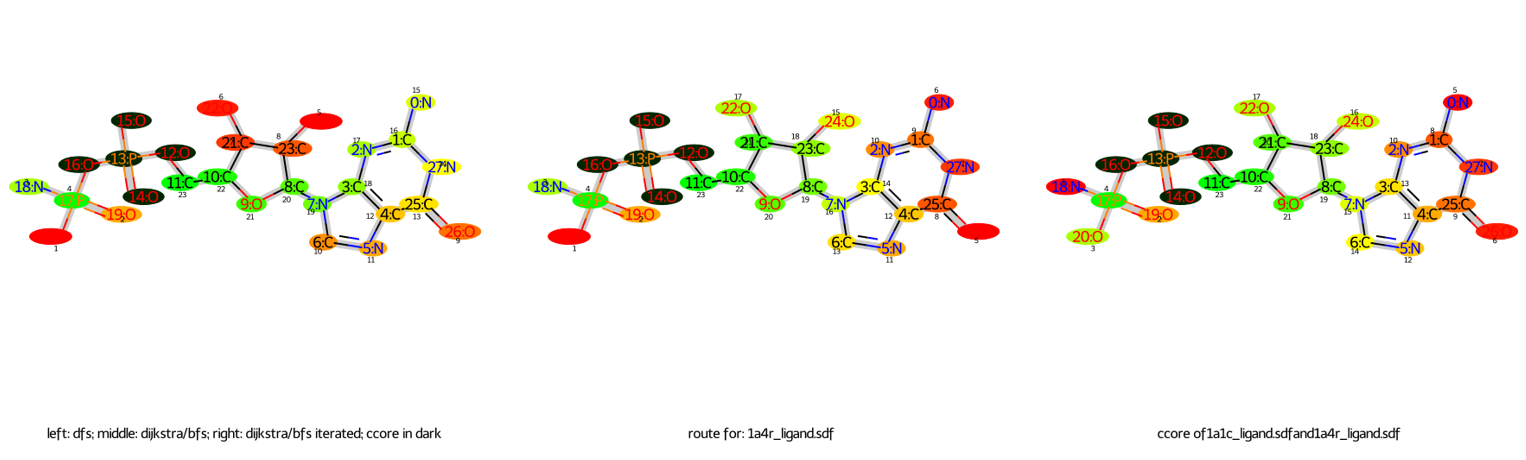
\includegraphics[scale=0.4]{2ring_example2}\caption{left: dfs-algorithm; right: bfs-algorithm; common core in dark}

\end{figure}
